%  Created by Branden Stone on 2015-01-15.
%  Copyright (c) 2015 Branden Stone. All rights reserved.
%--------------------------------------------------------
\documentclass{article}


%---------------------------
% Packages
%---------------------------
\usepackage{amssymb, amsmath, latexsym, amsfonts, amsthm, mathrsfs} % Standard packages that are nice to have.
\usepackage{amsrefs} % Allows for easy referencing and citations.
\usepackage{verbatim} % Needed for \begin{comment} \end{comment}.
\usepackage[text={6in,9in},centering]{geometry} % Defines the dimensions of the text body.
\usepackage[colorlinks=true]{hyperref} % Allows for use of hyperlinks.
%\usepackage[doublespacing]{setspace} % Makes the document double spaced.
\usepackage[pdftex]{graphicx} % Allows for \includegraphics
\usepackage{enumerate} % Allows for easy modification of lists

\renewcommand{\arraystretch}{1.5}

%----------------------------
% Title and Author
%----------------------------

\title{Math 390 Homework 9}
\author{Due Friday, May 6}
\date{}


%----------------------------
% Main Document Body
%----------------------------

\begin{document}


%-------------------------------------------------------------
% Front Matter: This is where you can add a table of contents,
% preface, list of figures, ETC. for this template we will 
% only create a title and author name with `\maketitle'
%-------------------------------------------------------------

\maketitle

\setlength{\parindent}{0em} % Sets indentation of new paragraph
\setlength{\parskip}{1em} % Sets space between paragraphs

%-------------------------------------------------------------
% Document Body: Essentially this is where you place the 
% content of your document. To use this template, just delete
% all of the text between here and the Bibliography Section.
% Then type whatever you desire.
%-------------------------------------------------------------


Solutions should be written \LaTeX\ or Markdown and converted to a PDF. You are encouraged to work with others
on the assignment, but you should write up your own solutions independently. This means no copy pasting. You should
reference all of your sources, including your collaborators. 

\begin{enumerate}

\item \begin{enumerate}
	\item Let $G = (V_1,V_2)$ be a cubic bipartite graph. Show that there is a complete matching from $V_1$ to $V_2$ as well as a complete matching from $V_2$ to $V_1$. (I.e. there is a one-to-one correspondence from $V_1$ onto $V_2$.)
	\item Show Tutte's 5-flow conjecture is true for cubic bipartite graphs. 
\end{enumerate}

\item Let $G$ be a simple graph that is not a null graph. Prove that the sum of the coefficients of $P_G(k)$ is 0. (Hint: When a function is a polynomial, how can one obtain the sum of the coefficients?)

\item The wheel graph $W_n$ is the $n$-vertex graph consisting of a cycle with $n-1$ vertices and an additional vertex that is adjacent to all of the vertices in the cycle. The wheel graphs $W_4$, $W_5$, and $W_6$ are shown below:
\begin{center}
	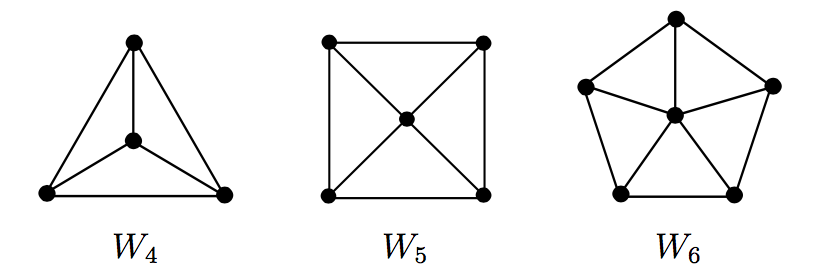
\includegraphics[width=.6\textwidth]{wheelpic.png}
\end{center}
Determine the chromatic polynomial of $W_n$ for $n\geqslant 4$. Prove your answer.

\item An {\bf infinite graph} is a graph $G$ where both the vertex set $V(G)$ and the edge set $E(G)$ are infinite. (In Edition 4 of the textbook, see Section 16 for more information about infinite graphs. In Edition 5 of the textbook, see pages 24, 38, and 44.)
\begin{enumerate}
	\item Find an Eulerian trail in the infinite square lattice. (The infinite square lattice is Figure 16.1 in Edition 4 and Figure 1.45 in Edition 5 of the textbook.)
	\item Give an example of a connected infinite graph in which every vertex has even degree, but the graph is not Eulerian.
\end{enumerate}




\end{enumerate}




\end{document}